\subsection{Route-Improvement Algorithm}
\label{subsec:03:rialgo}

The \emph{Route-Improvement Algorithm} (R-I-Algorithm) does not generate a path.
Rather, it takes a pre-existing path as input and tries to improve upon it.
It therefore can be used in conjunction with any path-generating algorithm.
Improving paths is done using three methods.

\begin{wrapfigure}{r}{0.45\textwidth}
	\centering
	\scalebox{0.78}{
		\begin{tikzpicture}[vertex/.style={draw}]
			\foreach \a in {1,...,6}{
					\draw (216-\a*360/10: 2.6cm) node (\a) {$v_\a$};
				}
			\draw[->] (1) -- (2);
			\draw[->] (2) -- (3);
			\draw[->] (3) -- (4);
			\draw[->] (4) -- (5);
			\draw[->] (5) -- (6);
		\end{tikzpicture}
		\vspace{-10pt}
	}
	\caption{A path generated by some algorithm.}
	\label{fig:03:rialgoreorderpath}
\end{wrapfigure}

\begin{enumerate}
	\itemsep0em
	\item Reorder nodes in the path.
	\item Introduce new nodes
	\item Replace one node with another.
\end{enumerate}

For this section, we will use variations of the example path in \cref{fig:03:rialgoreorderpath}.
In the following, inserted sections of the path are blue, and removed sections of the path are red and removed edges are additionally dotted.

\subsubsection{Reordering Nodes}
\label{subsubsec:03:reorder}

The first operation is to reorder nodes within a path by swapping two nodes.
While this will not increase a path's score, one hopes that it will reduce the path's total weight.

There are two types of swaps between two nodes $v_i$ and $v_j$.
\begin{enumerate}
	\itemsep0em
	\item Swap $v_i$ and $v_j$ keeping the order of nodes between them.
	\item Swap $v_i$ and $v_j$ and reverse the order of nodes between them.
\end{enumerate}
If any of the two types of swaps decreases the weight, the better swap is applied to the path.

If we swap nodes $v_2$ and $v_5$ and keep the order of the nodes in between them
then the resulting path is $v_1, v_5, v_3, v_4, v_2, v_6$. (see \cref{fig:03:rialgoreorderkeep})
If instead we reverse the order of the nodes between $v_5$ and $v_2$, this results in the path $v_1, v_5, v_4, v_3, v_2, v_6$. (see \cref{fig:03:rialgoreorderreverse})

\begin{figure}
	\centering
	\begin{subfigure}{0.45\textwidth}
		\centering
		\scalebox{0.78}{
			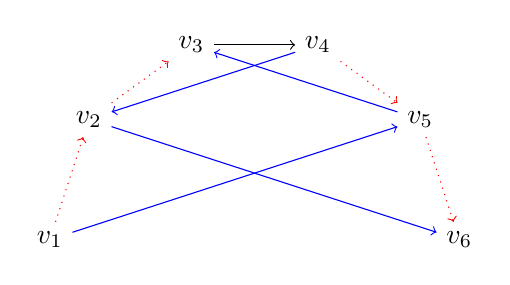
\begin{tikzpicture}[vertex/.style={draw}]
				\foreach \a in {1,...,6}{
						\draw (216-\a*360/10: 2.6cm) node (\a) {$v_\a$};
					}
				\draw[red,dotted,->] (1) -- (2);
				\draw[red,dotted,->] (2) -- (3);
				\draw[blue,->] (1) -- (5);
				\draw[blue,->] (5) -- (3);
				\draw[->] (3) -- (4);
				\draw[blue,->] (4) -- (2);
				\draw[blue,->] (2) -- (6);
				\draw[red,dotted,->] (4) -- (5);
				\draw[red,dotted,->] (5) -- (6);
			\end{tikzpicture}
		}
		\caption{Swapping $v_2$ and $v_5$, keeping the order of the nodes in between.}
		\label{fig:03:rialgoreorderkeep}
	\end{subfigure}
	\begin{subfigure}{0.45\textwidth}
		\centering
		\scalebox{0.78}{
			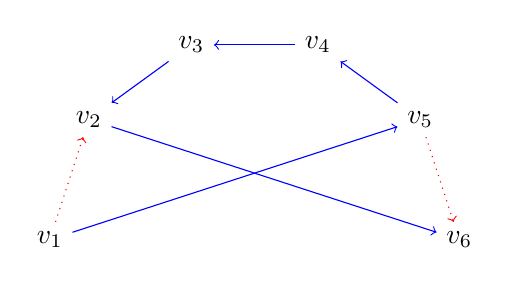
\begin{tikzpicture}[vertex/.style={draw}]
				\foreach \a in {1,...,6}{
						\draw (216-\a*360/10: 2.6cm) node (\a) {$v_\a$};
					}
				\draw[red,dotted,->] (1) -- (2);
				\draw[red,dotted,->] (5) -- (6);
				\draw[blue,->] (1) -- (5);
				\draw[blue,->] (5) -- (4);
				\draw[blue,->] (4) -- (3);
				\draw[blue,->] (3) -- (2);
				\draw[blue,->] (2) -- (6);
			\end{tikzpicture}
		}
		\caption{Swapping $v_2$ and $v_5$, \emph{reversing} the order of the nodes in between.}
		\label{fig:03:rialgoreorderreverse}
	\end{subfigure}
	\caption{The reordering phase of the R-I-Algorithm.}
	\label{fig:03:rialgoreorder}
\end{figure}

\subsubsection{Introduction of new Nodes}

\begin{wrapfigure}{r}{0.45\textwidth}
	\centering
	\begin{tikzpicture}[vertex/.style={draw}]
		\foreach \a in {1,2,4,5,6}{
				\draw (216-\a*360/10: 2.6cm) node (\a) {$v_\a$};
			}
		\draw[blue] (216-3*360/10: 2.6cm) node (3) {$v_3$};
		\draw[blue,->] (2) -- (3);
		\draw[blue,->] (3) -- (4);
		\draw[->] (1) -- (2);
		\draw[red,dotted,->] (2) -- (4);
		\draw[->] (4) -- (5);
		\draw[->] (5) -- (6);
	\end{tikzpicture}
	\caption{Inserting $v_3$ into the path.}
	\label{fig:03:rialgoinsert}
\end{wrapfigure}

This operation inserts a new node into the path.
For each unvisited node, we determine the position in the path where if the node was inserted the increase in cost is minimized.
If the set of possible insertions is determined, the position that increases the cost the least is chosen.
Of course, only insertions that do not violate $T_{max}$ are allowed.
In contrast to the previous section, this operation does not decrease the cost of the path, but can only increase score.
An example is depicted in \cref{fig:03:rialgoinsert} where $v_3$ is inserted into the path.

\subsubsection{Replacing a Node}

\begin{wrapfigure}{r}{0.45\textwidth}
	\centering
	\begin{tikzpicture}[vertex/.style={draw}]
		\foreach \a in {1,3,4,6}{
				\draw (216-\a*360/10: 2.6cm) node (\a) {$v_\a$};
			}
		\draw[blue] (216-2*360/10: 2.6cm) node (2) {$v_2$};
		\draw[red] (216-5*360/10: 2.6cm) node (5) {$v_5$};
		\draw[blue,->] (1) -- (2);
		\draw[blue,->] (2) -- (3);
		\draw[red,dotted,->] (1) -- (3);
		\draw[->] (3) -- (4);
		\draw[red,dotted,->] (4) -- (5);
		\draw[blue,->] (4) -- (6);
		\draw[red,dotted,->] (5) -- (6);
	\end{tikzpicture}
	\caption{Inserting $v_2$ and removing $v_5$.}
	\label{fig:03:rialgoreplace}
\end{wrapfigure}

This approach inserts an unvisited node into the path while at the same time removing another node from the path.
Like in the previous step, for each unvisited node $v \in V \backslash P$, we determine the position in the path which would increase the cost by the least amount if the node was inserted.
Note that here we do \emph{not} care about violations of $T_{max}$.
We additionally determine a visited node $w \in P \backslash \{v_1, v_n\}$ which, if removed, would free up enough capacity to insert $v$ at the previously determined position.
Out of all the nodes that fulfill this condition, we pick the one with the smallest score.
This yields possibly multiple pairs of nodes $(v, w)$, the unvisited node $v$ to insert and the visited node $w$ to remove.
Out of these we pick the most profitable pair.
An example is depicted in \cref{fig:03:rialgoreplace} in which $v_2$ is replaced with $v_5$.

\subsubsection{Generalizing to non-Euclidean inputs}

Since this algorithm does not make any assumptions about its input, except for graph completeness it should work on any graph that is complete.

